\documentclass[10pt,aspectratio=169,utf8]{beamer}

% ctex fontset=auto 自动适配系统字体: macOS 用 ST 系列, Linux 用 Fandol 系列
\usepackage{ctex}
\IfFontExistsTF{Heiti SC}{\setCJKmonofont{Heiti SC}}{}  % 等宽字体: macOS 用黑体, 否则用 ctex 默认

\usepackage{graphicx}
\usepackage{xcolor}
\usepackage{booktabs}
\usepackage{tikz}
\usetikzlibrary{positioning}
\usepackage{fontawesome5}
\usepackage{hyperref}
\usepackage{fancyvrb}

\usetheme{Copenhagen}
\usecolortheme{default}

\definecolor{mygreen}{RGB}{34,139,34}
\definecolor{myblue}{RGB}{0,102,204}
\definecolor{myred}{RGB}{220,50,50}
\definecolor{mygray}{RGB}{120,120,120}
\definecolor{mybg}{RGB}{248,248,252}

\setbeamercolor{background canvas}{bg=mybg}
\setbeamercolor{frametitle}{bg=mybg,fg=myblue}
\setbeamercolor{title}{fg=myblue}
\setbeamercolor{subtitle}{fg=mygray}
\setbeamercolor{block title}{bg=myblue,fg=white}
\setbeamercolor{block body}{bg=white}
\setbeamercolor{alerted text}{fg=myred}

\setbeamertemplate{itemize item}{\textbullet}
\setbeamertemplate{itemize subitem}{--}
\setbeamertemplate{footline}[frame number]
\setbeamertemplate{section in toc}{\inserttocsectionnumber.~\inserttocsection}

\DefineVerbatimEnvironment{code}{Verbatim}{fontsize=\tiny,frame=single}

\title{\textbf{upctl-compose 用户手册}\\[2pt]{\normalsize 本地部署 \& AI Agent 自动处理指南}}
\subtitle{\small 基于AI Agent的全自动开发平台}
\author{鉬馨玥翼}
\date{\today}

\begin{document}

\begin{frame}[plain]
  \titlepage
\end{frame}

\begin{frame}[shrink=10]{目录}
  \tableofcontents
\end{frame}

% ============================================
\section{系统架构}
% ============================================

\begin{frame}[shrink=10]{系统架构总览}
  \begin{center}
    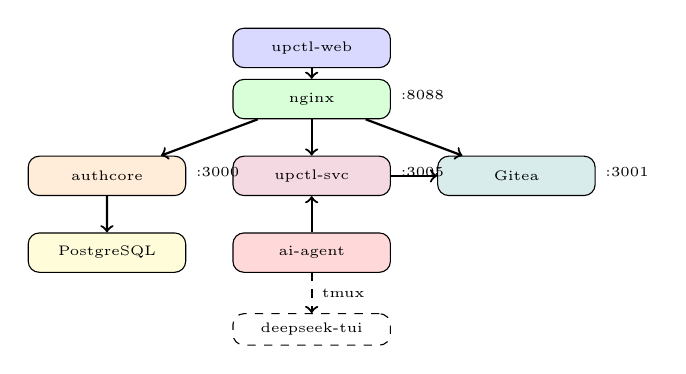
\begin{tikzpicture}[
      svc/.style={rectangle, draw, rounded corners, minimum width=2cm, minimum height=0.5cm, align=center, font=\tiny},
      scale=0.65
    ]
      \node[svc, fill=blue!15] (web) at (0, 3.5) {upctl-web};
      \node[svc, fill=green!15] (nginx) at (0, 2.5) {nginx};
      \node[svc, fill=orange!15] (auth) at (-4, 1) {authcore};
      \node[svc, fill=purple!15] (svc) at (0, 1) {upctl-svc};
      \node[svc, fill=teal!15] (gitea) at (4, 1) {Gitea};
      \node[svc, fill=yellow!15] (pg) at (-4, -0.5) {PostgreSQL};
      \node[svc, fill=red!15] (ai) at (0, -0.5) {ai-agent};
      \node[draw, dashed, rounded corners, minimum width=2cm, minimum height=0.4cm, font=\tiny] (ds) at (0, -2) {deepseek-tui};
      \draw[->,thick] (web) -- (nginx);
      \draw[->,thick] (nginx) -- (auth);
      \draw[->,thick] (nginx) -- (svc);
      \draw[->,thick] (nginx) -- (gitea);
      \draw[->,thick] (svc) -- (gitea);
      \draw[->,thick] (ai) -- (svc);
      \draw[->,thick] (auth) -- (pg);
      \draw[->,thick,dashed] (ai) -- (ds) node[midway, right, font=\tiny] {tmux};
      \node[font=\tiny, right] at ([yshift=2pt]nginx.east) {:8088};
      \node[font=\tiny, right] at ([yshift=2pt]auth.east) {:3000};
      \node[font=\tiny, right] at ([yshift=2pt]svc.east) {:3005};
      \node[font=\tiny, right] at ([yshift=2pt]gitea.east) {:3001};
    \end{tikzpicture}
  \end{center}
  \vspace{2pt}
  \begin{table}
    \fontsize{7}{9}\selectfont
    \begin{tabular}{lcl}
      \toprule
      服务 & 端口 & 作用 \\
      \midrule
      nginx & 8088 & 反向代理，路由到各后端 \\
      authcore & 3000 & 身份认证，JWT 签发 \\
      upctl-svc & 3005 & 工单 CRUD API \\
      upctl-web & (nginx 内) & Vue 3 前端 \\
      ai-agent & --- & 轮询 Gitea + tmux 托管 deepseek-tui \\
      Gitea & 3001 & 代码托管+工单+CI \\
      PostgreSQL & 5432 & 数据库 \\
      \bottomrule
    \end{tabular}
  \end{table}
\end{frame}

\begin{frame}[shrink=10]{AI Agent 工作流程}
  \begin{center}
    \begin{tikzpicture}[node distance=0.5cm, auto]
      \tikzset{block/.style={rectangle, draw, rounded corners, minimum width=1.3cm, minimum height=0.4cm, align=center, font=\tiny}}
      \node[block, fill=green!20] (poll) {轮询 approved};
      \node[block, fill=blue!20, right=of poll] (label) {加 in\_progress};
      \node[block, fill=orange!20, right=of label] (llm) {deepseek-tui};
      \node[block, fill=purple!20, below=of llm] (comment) {评论结果};
      \node[block, fill=gray!20, left=of comment] (remove) {移除 label};
      \node[block, fill=red!20, left=of remove] (close) {关闭};
      \draw[->,thick] (poll) -- (label);
      \draw[->,thick] (label) -- (llm);
      \draw[->,thick] (llm) -- (comment);
      \draw[->,thick] (comment) -- (remove);
      \draw[->,thick] (remove) -- (close);
      \draw[->,thick,dashed] ([yshift=-0.15cm]close.south) -- ++(0,-0.35) -| (poll.west);
    \end{tikzpicture}
  \end{center}
  \vspace{2pt}
  \begin{exampleblock}{关键特征}
    \footnotesize
    每 5 分钟轮询 {\small |} tmux 托管 deepseek-tui {\small |} 自动评论并关闭
  \end{exampleblock}
\end{frame}

% ============================================
\section{本地部署}
% ============================================

\begin{frame}{环境要求}
  \small
  \begin{columns}[T]
    \column{0.48\textwidth}
    \textbf{软件要求}
    \begin{itemize}
      \item Docker 24.0+, Compose 2.24+
      \item Git
    \end{itemize}
    \textbf{端口占用}\\
    \texttt{5432} PostgreSQL \quad \texttt{3000} authcore\\
    \texttt{3001} Gitea \quad \texttt{3005} upctl-svc\\
    \texttt{8088} nginx \quad \texttt{2222} Gitea SSH

    \column{0.48\textwidth}
    \textbf{推荐配置}
    \begin{itemize}
      \item CPU 4 核 +、内存 8 GB +
      \item 需访问 GitHub + DeepSeek API
    \end{itemize}
    \textcolor{myred}{\textbf{注意：}} Docker Desktop 需配置 \texttt{no\_proxy}（已内置）
  \end{columns}
\end{frame}

\begin{frame}[fragile]{克隆与启动}
  \begin{columns}[T]
    \column{0.48\textwidth}
    \begin{block}{1. 克隆}
      \begin{code}
git clone https://github.com/
  alchemy-studio/upctl-compose.git
cd upctl-compose
      \end{code}
    \end{block}
    \begin{block}{2. 启动}
      \begin{code}
docker compose up -d
docker compose ps
      \end{code}
    \end{block}

    \column{0.48\textwidth}
    \begin{block}{启动日志}
      \tiny
      authcore: Running migration...\\
      \relax\ [authcore] Starting htyuc...\\
      数据库连接池初始化 OK\\
      upctl-svc: starting on port 3005\\
      ai-agent: Setting up workspace...\\
      \relax\ Starting tmux session...
    \end{block}
  \end{columns}
\end{frame}

\begin{frame}[fragile]{初始化 Gitea}
  \begin{columns}[T]
    \column{0.48\textwidth}
    \begin{block}{等待 Gitea}
      \begin{code}
until curl -sf localhost:3001/api/v1/version
do sleep 3; done
      \end{code}
    \end{block}
    \begin{block}{初始化}
      \begin{code}
docker compose exec ai-agent \
  python3 /app/setup-gitea.py
      \end{code}
    \end{block}

    \column{0.48\textwidth}
    \begin{block}{创建内容}
      \footnotesize
      组织 \texttt{weli} + 仓库 \texttt{tickets}\\
      标签：approved(1) / in\_progress(2) / blocked(3)
    \end{block}
    \begin{exampleblock}{管理界面}
      \footnotesize
      \url{http://localhost:3001} \\
      用户 \texttt{ai-bot / ai-bot-dev-pass}
    \end{exampleblock}
  \end{columns}
\end{frame}

\begin{frame}[fragile]{AI 代理配置}
  \begin{columns}[T]
    \column{0.48\textwidth}
    \begin{block}{.env 文件}
      \begin{code}
DEEPSEEK_API_KEY=sk-your-key
DEEPSEEK_API_BASE=https://api.deepseek.com
DEFAULT_MODEL=deepseek-v4-flash
      \end{code}
    \end{block}
    \begin{block}{重启}
      \begin{code}
docker compose up -d ai-agent
      \end{code}
    \end{block}

    \column{0.48\textwidth}
    \begin{exampleblock}{验证部署}
      \footnotesize
      \begin{code}
curl -sf localhost:8088/ | head -c 200
curl -sf localhost:3005/   # upctl-svc
curl -sf localhost:3000/   # AuthCore
      \end{code}
    \end{exampleblock}
  \end{columns}
\end{frame}

% ============================================
\section{使用指南}
% ============================================

\begin{frame}{登录页面}
  \begin{columns}[T]
    \column{0.55\textwidth}
    访问 \url{http://localhost:8088}
    \begin{itemize}
      \item 开发模式显示用户名密码登录表单
      \item 使用 \texttt{demo / demo123} 登录
      \item AuthCore 验证后直接签发 JWT
      \item 登录后跳转工单列表
    \end{itemize}
    \vspace{4pt}
    \textcolor{myblue}{认证流程：} 前端 $\to$ nginx $\to$ authcore 验证密码 $\to$ JWT

    \column{0.43\textwidth}
    \includegraphics[width=\textwidth]{screenshots/01-login-page.png}
  \end{columns}
\end{frame}

\begin{frame}{工单列表 \& 详情}
  \begin{columns}[T]
    \column{0.55\textwidth}
    \textbf{列表页：} 标签页切换 / 卡片显示标题+状态\\
    \textbf{详情页：} 标题+编号 / 状态标签 / 评论区\\[4pt]
    AI 处理结果格式：\\
    \texttt{\#\# Processing result}\\
    \texttt{\{AI 总结\}}\\
    \texttt{--- *Processed by DeepSeek Agent*}

    \column{0.43\textwidth}
    \includegraphics[width=\textwidth]{screenshots/02-ticket-list.png}
    \vspace{4pt}
    \includegraphics[width=\textwidth]{screenshots/03-ticket-detail.png}
  \end{columns}
\end{frame}

\begin{frame}{Gitea 后台}
  \begin{columns}[T]
    \column{0.55\textwidth}
    地址 \url{http://localhost:3001}\\
    用户 \texttt{ai-bot / ai-bot-dev-pass}\\
    仓库 \texttt{weli/tickets}\\[4pt]
    标签说明：
    \begin{itemize}
      \item \texttt{approved} --- AI 自动处理
      \item \texttt{in\_progress} --- 处理中
      \item \texttt{blocked} --- 阻塞
    \end{itemize}

    \column{0.43\textwidth}
    \includegraphics[width=\textwidth]{screenshots/04-gitea-issues.png}
  \end{columns}
\end{frame}

\begin{frame}[fragile]{AI Agent 自动处理}
  \begin{columns}[T]
    \column{0.55\textwidth}
    系统部署完成后，AI Agent 自动开始轮询：\\[4pt]
    \begin{enumerate}
      \item 在 Gitea 创建工单并打 \texttt{approved} 标签
      \item ai-agent 每 5 分钟轮询发现新工单
      \item 自动调用 DeepSeek API 处理
      \item 评论结果并关闭工单
    \end{enumerate}
    \vspace{4pt}
    也可手动启动即时处理：\\[4pt]
    \texttt{\$\ docker\ compose\ exec\ ai-agent\ \textbackslash}\\
    \texttt{\qquad python3\ /app/poll\_worker.py\ --once}

    \column{0.43\textwidth}
    \includegraphics[width=\textwidth]{screenshots/05-ticket-list-with-data.png}
    \vspace{4pt}
    \tiny ai-agent 自动轮询日志：\\
    \texttt{Processing issue \#185}\\
    \texttt{DeepSeek response received}\\
    \texttt{close \#185: 200 -- completed}
  \end{columns}
\end{frame}

% ============================================
\section{组件日志}
% ============================================

\begin{frame}[fragile]{各组件日志解读}
  \begin{columns}[T]
    \column{0.48\textwidth}
    \begin{block}{authcore 启动}
      \tiny
      Running migration 2022-02-14-124946\\
      \relax Running migration 2026-05-02-082153\\
      \relax\ [authcore] Starting htyuc...\\
      全局数据库连接池初始化 OK
    \end{block}
    \begin{block}{upctl-svc}
      \tiny
      [upctl-svc] starting on port 3005\\
      \relax [upctl-svc] listening on 0.0.0.0:3005
    \end{block}

    \column{0.48\textwidth}
    \begin{block}{ai-agent 轮询}
      \tiny
      poll\_worker started -- interval=300s\\
      No approved issues found.\\
      No work. Sleeping 300s...
    \end{block}
    \begin{block}{ai-agent 处理}
      \tiny
      Processing issue \#185: 添加dependbot\\
      add\_label \#185: 200\\
      DeepSeek response received (594 chars)\\
      add\_comment \#185: 200\\
      close \#185: 200 -- completed
    \end{block}
  \end{columns}
\end{frame}

\begin{frame}[fragile]{tmux 运行时 \& 容器状态}
  \begin{columns}[T]
    \column{0.48\textwidth}
    \begin{block}{tmux 调试}
      \tiny
      \# 进入 session\\
      docker compose exec ai-agent \\
      \relax\ \ tmux attach -t deepseek-agent\\
      \# 查看输出\\
      docker compose exec ai-agent \\
      \relax\ \ tmux capture-pane -t deepseek-agent -p
    \end{block}

    \column{0.48\textwidth}
    \begin{block}{docker compose ps}
      \tiny
      NAME                  STATUS\\
      ai-agent   Up (healthy)\\
      authcore   Up\\
      gitea      Up\\
      postgres   Up (healthy)\\
      upctl-svc  Up\\
      upctl-web  Up
    \end{block}
    \begin{alertblock}{使用 tmux send-keys 注入命令}
      \tiny
      可在不进入交互模式的情况下向 agent 发送命令
    \end{alertblock}
  \end{columns}
\end{frame}

% ============================================
\section{容器内 CI}
% ============================================

\begin{frame}{Gitea Issue 自动处理流程}
  \small
  \begin{columns}[T]
    \column{0.55\textwidth}
    本系统使用 \textbf{Gitea + ai-agent} 实现工单自动处理，无需外部 CI：

    \begin{enumerate}
      \item 创建工单，标记 \texttt{approved}
      \item ai-agent 每 5min 轮询 Gitea API
      \item 发现 \texttt{approved} 工单 $\to$ 加 \texttt{in\_progress}
      \item tmux send-keys 注入工单内容到 \texttt{deepseek-tui} 对话
      \item deepseek-tui 与 \texttt{api.deepseek.com} 交互生成回复
      \item tmux capture-pane 读取回复内容
      \item 评论结果到工单
      \item 移除 \texttt{in\_progress} + 关闭工单
    \end{enumerate}

    \column{0.43\textwidth}
    \includegraphics[width=\textwidth]{screenshots/04-gitea-issues.png}
  \end{columns}
\end{frame}

\begin{frame}[fragile]{ai-agent 工作日志}
  \begin{columns}[T]
    \column{0.48\textwidth}
    \begin{block}{启动阶段}
      \tiny
      Setting up workspace...\\
      Starting tmux session...\\
      Starting poll worker...\\
      poll\_worker started -- interval=300s
    \end{block}
    \begin{block}{空闲状态}
      \tiny
      No approved issues found.\\
      No work. Sleeping 300s...
    \end{block}

    \column{0.48\textwidth}
    \begin{block}{处理工单}
      \tiny
      Processing issue \#185: 添加dependbot\\
      add\_label \#185: 200\\
      DeepSeek response received (594 chars)\\
      add\_comment \#185: 200\\
      close \#185: 200 -- completed
    \end{block}
  \end{columns}
  \vspace{4pt}
  \textcolor{myblue}{关键技术：} Python 轮询 | tmux send-keys 注入 | deepseek-tui CLI | Gitea API
\end{frame}

\begin{frame}[fragile]{deepseek-tui 验证}
  \begin{columns}[T]
    \column{0.48\textwidth}
    \begin{block}{tmux 终端}
      \tiny
      root@ai-agent:/app/workspace\# deepseek-tui --version\\
      deepseek-tui (npm wrapper) v0.8.22\\
      binary version: v0.8.22\\
      repo: git+https://github.com/Hmbown/DeepSeek-TUI.git
    \end{block}

    \column{0.48\textwidth}
    \begin{block}{实际运行日志}
      \tiny
      docker compose logs ai-agent --tail 5\\
      {[}ai-agent{]} Setting up workspace...\\
      {[}ai-agent{]} Starting tmux session...\\
      {[}ai-agent{]} Starting poll worker...\\
      {[}2026-05-09{]} poll\_worker started -- interval=300s\\
      {[}2026-05-09{]} No work. Sleeping 300s...
    \end{block}
  \end{columns}
  \vspace{4pt}
  \textcolor{myblue}{注意：} 日志已脱敏，无密文泄露
\end{frame}

% ============================================
\section{故障排除}
% ============================================

\begin{frame}{常见问题}
  \fontsize{7.5}{9.5}\selectfont
  \begin{tabular}{p{3.5cm}p{3cm}p{5.5cm}}
    \toprule
    问题 & 原因 & 解决 \\
    \midrule
    POOL\_SIZE must be set & authcore 缺变量 & 加 POOL\_SIZE: "10" \\
    JWT\_KEY not set & upctl-svc 缺变量 & 加 JWT\_KEY 环境变量 \\
    Gitea API 404 & 路径错误 & 用 /api/v1/ 根路径 \\
    前端白屏/JS 404 & 资源未构建 & docker compose build upctl-web \\
    ai-agent 未连 DeepSeek & 缺 API Key & 配置后重启 \\
    容器间连接失败 & Docker Desktop 代理 & 设置 no\_proxy（已内置） \\
    Playwright 401 & JWT 格式 & ts 无 Z 后缀 \\
    remove\_label 404 & 标签 ID & approved=1, in\_progress=2 \\
    \bottomrule
  \end{tabular}
\end{frame}

\begin{frame}{总结}
  \begin{center}
    \vspace{0.8cm}
    {\Large\bfseries upctl-compose}
    \vspace{0.2cm}
    {\normalsize AI Agent 驱动的全自动开发平台}

    \vspace{0.3cm}
    \begin{block}{核心能力}
      \centering
      \faDocker\ 6 容器一键部署 \qquad
      \faRobot\ DeepSeek 自动处理 \qquad
      \faCheckCircle\ Playwright 全链路测试
    \end{block}

    \vspace{0.3cm}
    \texttt{git clone https://github.com/alchemy-studio/upctl-compose.git \&\& cd upctl-compose \&\& docker compose up -d}
  \end{center}
\end{frame}

\begin{frame}[plain]
  \begin{center}
    \vspace{3cm}
    {\Huge \textcolor{myblue}{\textbf{Thank You}}}

    \vspace{2cm}
    {\Large \textbf{鉬馨玥翼}}

    \vspace{0.8cm}
    {\Large \url{https://github.com/alchemy-studio/upctl-compose}}
  \end{center}
\end{frame}

\end{document}
